\documentclass[conference]{IEEEtran}

% Write an eight page technical paper describing your project in the style of an IEEE Visualization Technical Paper (other formats may be acceptable with pre-approval).

% Sections you should plan to include are: abstract, introduction, related work (adapt your literature review for this), implementation, results, future directions, and references.

% Your paper should include figures and images as appropriate.

% A complete draft of your paper, including figures and images, must be submitted in advance of the final paper deadline.

% Your draft should be a complete paper that is as strong and polished as you can make it.

% Aim for something that you believe is ready for submission to a conference or journal.

% The course instructor will serve as reviewer for these papers and make suggestions as to how they might be improved.

% You may submit earlier, not necessarily complete, drafts of your paper if you would like feedback earlier in the writing process.

% Correct spelling and grammar count in all submitted work, so check them before you hand anything in.

\usepackage{epsfig}

% Example figure
%\begin{figure}[ht]
% \centering
% \includegraphics[scale=.8]{old.png}
% \caption{}
% \label{old}
% \end{figure}


\hyphenation{SwarmVis}

\begin{document}

\title{SwarmVis: a Tool for Visualizing Swarm Systems}

\author{\IEEEauthorblockN{Don Miner}
\and
\IEEEauthorblockN{Niels Kasch}
}
\maketitle


\begin{abstract}
In this paper, we provide an overview of SwarmVis, a tool for
visualizing swarm systems. SwarmVis integrates several visualization
techniques to create informative still images and videos of swarm
systems moving through two- and three- dimensional space. SwarmVis
allows swarm researchers to observe characteristics of swarm systems by
visualizing information about such systems. We provide an overview of
the types of information relevant to current swarm research and explain,
in detail, the capabilities of SwarmVis to visualize this information.
Finally, we use a case study to
demonstrate how SwarmVis can be used to analyze both the local agent and
global swarm behaviors of multi-agent systems.

\end{abstract}

\section{Introduction}
A swarm system is a collection of autonomous agents that, as a group,
often exhibit some complex behavior.
Examples of these systems include: social animals (e.g. ants\cite{couzin2003sol}, schooling fish\cite{parrish2002sof}, migrating geese\cite{reynolds1987}), 
and multi-robot systems\cite{mondada2004sbn}\cite{mclurkin2004srt}.
Visualizing swarm systems (swarms) effectively is non-trivial task, partially due to the large number of individual agents contained.
The high density and chaotic motions of agents found in typical swarms amplify the complexity of swarm visualization.
Effective swarm visualizations are needed to provide insight into local (agent-level) and global (swarm-level) behavior.
A well defined set of visualization techniques in combination with an interactive exploratory tool provides
the facilities to allow researchers to gain these insights.


Simple visualization techniques have been used to plot the position of each agent in space.
An example of this technique, illustrating a Reynolds boid flock\cite{reynolds1987}, can be seen in Figure \ref{Intro} (left).
The image only shows the location of individual agents and does not convey important
information such as direction, velocity, and previous positions of the agents.
We have implemented \textit{SwarmVis}, a toolkit for visualizing swarms,
that goes beyond the simple plotting technique to increase the
expressiveness of swarm visualizations.
The toolkit aims to provide visualization techniques that allows researchers to interactively
investigate swarms in order to study interactions, fine-grained movements, and swarm behavior.
Figure \ref{Intro} (right) displays a swarm system with the addition of our trails visualization and conveys much more
information than Figure \ref{Intro} (left).

\begin{figure}[ht]
\centering
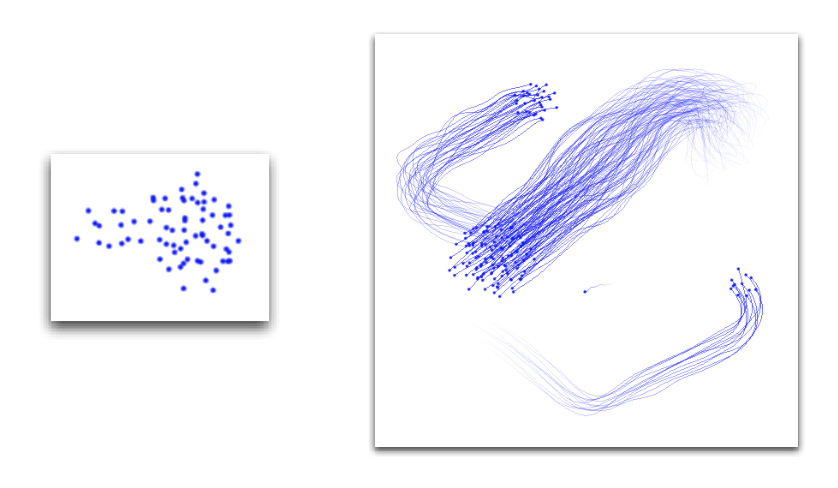
\includegraphics[scale=.55]{images/intro.pdf}
\caption{(Left) A basic visualization of a boid flock with agents are plotted as
points in space. The image only conveys positional and limited structural information.
(Right) A visualization of the boid flock using SwarmVis. Agent
position is augmented by a trail of significant length (right).
Important properties such as direction, velocity, structure, rotation,
and previous positions are all naturally conveyed.
}
\label{Intro}
\end{figure}

The goal of SwarmVis is to facilitate, through visualization, the detailed analysis of emergent behavior that results from swarm systems.
In order to satisfy this objective, we have created a software toolkit
with the following high-level application goals and requirements in mind:
\begin{itemize}
\item The toolkit shall visualize swarms using a series of still images (i.e. an animation)
embedded in an interactive user interface that has features such as pausing, slowing down and rewinding of frames.
\item Agent position, direction and velocity shall be conveyable through both still images and videos generated from the software.
\item The toolkit shall provide a variety of built-in visualization techniques that are useful in visualizing swarm systems.
\end{itemize}

In the next section, we discuss previous work in swarm system visualization,
some of which has provided inspirations for the techniques employed in SwarmVis.
Next, we discuss the implementation details of the visualizations and the user interface.
We conclude with a demonstration of the effectiveness of SwarmVis by using it to explore and analyze a swarm system.
A brief user guide for compiling, running and loading data in SwarmVis is provided in the appendix.


\section{Related Work}
Not much work has been done that specifically addresses the problem of creating effective swarm visualizations.
Most swarm visualizations in the literature are the result of swarm intelligence research. However, the literature does neither discuss the details of such visualizations nor their effectiveness. 

Comprehensive multi-agent and swarm system frameworks\cite{Luke}\cite{860347} have been created previously. Their priority is mainly on the simulation of the evolution of swarms not the visual representation of the process.
Some researchers have implemented visualization techniques for specific swarm domains,
such as the particle swarm optimization algorithm\cite{Secrest} and boid flocking\cite{reynolds1987}.
There have been several projects that used a swarm system paradigm to visualize a particular subset of information or domain, such as data variations\cite{1382896}, art\cite{Boyd}, evolutionary algorithms\cite{spector2005ecb}\cite{Spector02evolutionarydynamics},
flow\cite{10.1109/TVCG.2005.87}\cite{Merzkirch}, and source code commits\cite{codeswarm:website}.

Our work is partially inspired by the lack of a coherent collection of effective visualization techniques for swarm systems. We often draw inspiration from illustrations in papers concerned with swarm systems, but which are not directly related to visualization. In this section, we discuss two projects that have motivated particular features in SwarmVis.

\begin{figure}
\centering
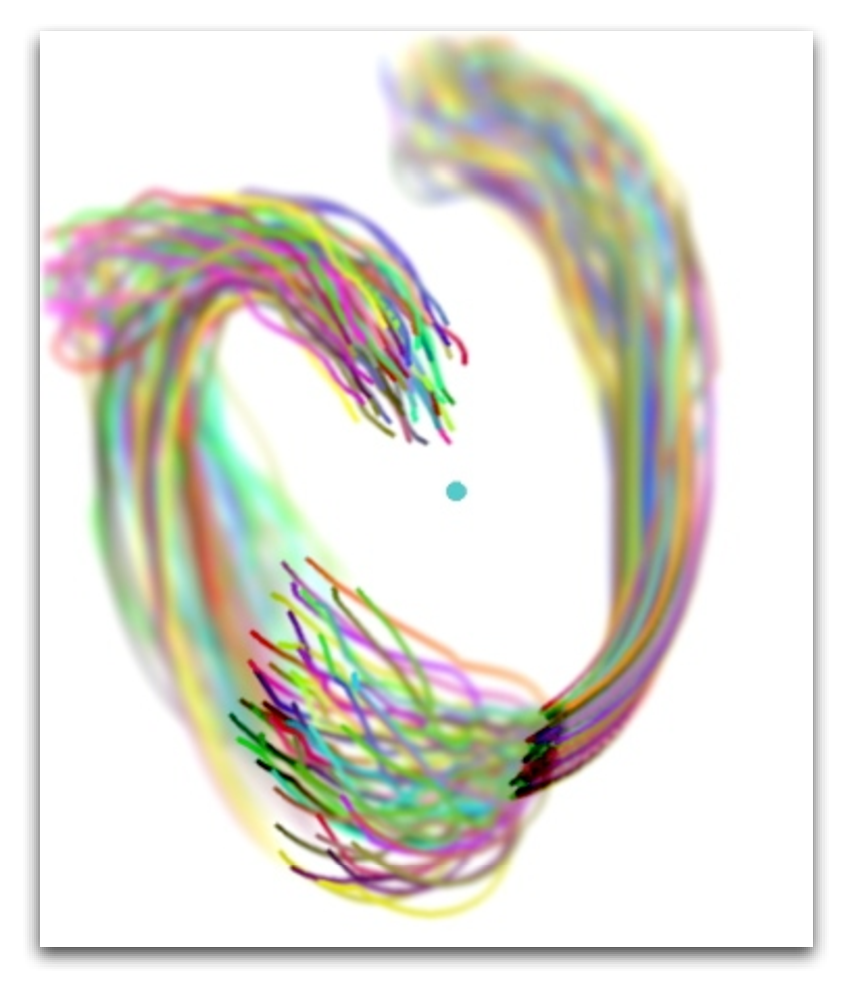
\includegraphics[scale=.3]{images/SwarmArt.pdf}
\caption{A visualization created by Boyd et al. with SwarmArt\cite{Boyd}.}
\label{SwarmArt}
\end{figure}

\subsection{SwarmArt}
SwarmArt\cite{Boyd} by Boyd et al. is a combination of science and art with the aim to create visually appealing swarms.
SwarmArt visualizes the positional data of a swarm by projecting individual agents as dots onto a 2D surface.
Motion is conveyed by incoorporating the previous positions of an agent into a trail that fades with time.
A sample image created with SwarmArt is shown in Figure \ref{SwarmArt}.
This work, among others\cite{codeswarm:website}, were inspirations for how we visualize agents as simple dots with fading trails
in SwarmVis.

\begin{figure}
\centering
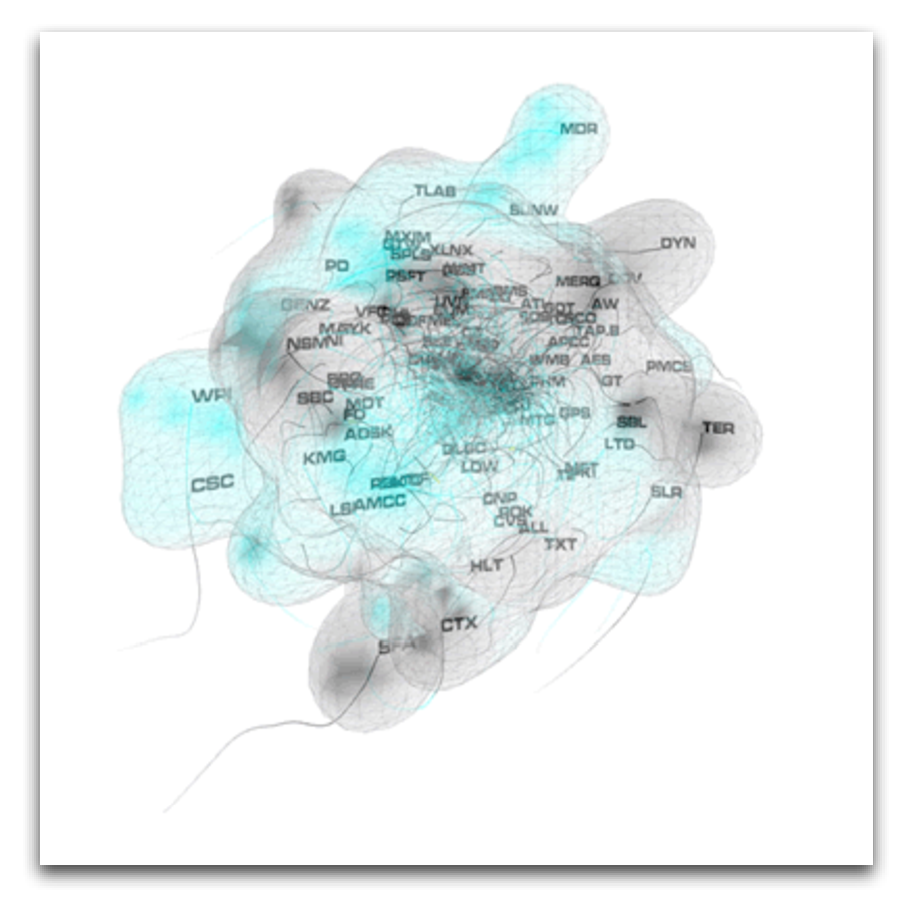
\includegraphics[scale=.4]{images/blob.pdf}
\caption{An ``information flocking" visualization created by Moere\cite{1382896}.}
\label{Blob}
\end{figure}

\subsection{Information Flocking}
Moere demonstrates how self-organization and behavior as seen in Reynolds' Boids can be used to show change of information over time\cite{1382896}. This method is dubbed {\em Information Flocking} and combines flocking behavior rules and clustering techniques to give users a unique perspective of changing data.
The domain presented in this paper and the method of information flocking are not directly relevant to our project.
However, the visualizations created by this author are smooth and can be considered visually appealing.
Each agent is a single particle in 3D space and its traveled path is depicted by a colored,
curved line that has gradually decreasing opacity from the head.
The trails are made smooth by using the {\em Catmull-Rom spline} algorithm,
which generates smoother trails than linear interpolation through the previous points the agent has visited.
The particles' color shows change in data values: blue and red for a decrease and increase, respectively.

In addition, the visualization may include an encompassing translucent ``blob'' that shows vicinity (data similarity). That is, if particles are in the same blob, they are in the same flock. This blob method also helps the user find outliers.
These blobs are generated with Marching Cubes; specifically a method called ``implicit surface polygonizer.'' Unfortunately, computing the blob is currently too computationally intensive to be displayed at every time step.
The author claims that this simulation was able to run in real time with 500 agents.

This work also motivated us in having SwarmVis show agents as a particle with a fading trail.
However, we decided against using a spline method since splines may obscure the actual path of an agent. Smothing the splines can - in some cases - introduce misleading representations of agent movements.
Moere's use of color in agent trails inspired a similar visualization in SwarmVis. In Section \ref{visualizations} we introduce a more intuitive mapping of information to trail color.
The ``blob" shown in this work is interesting and informative; in the future, we may implement this feature in SwarmVis.


\begin{figure*}[ht]
\centering
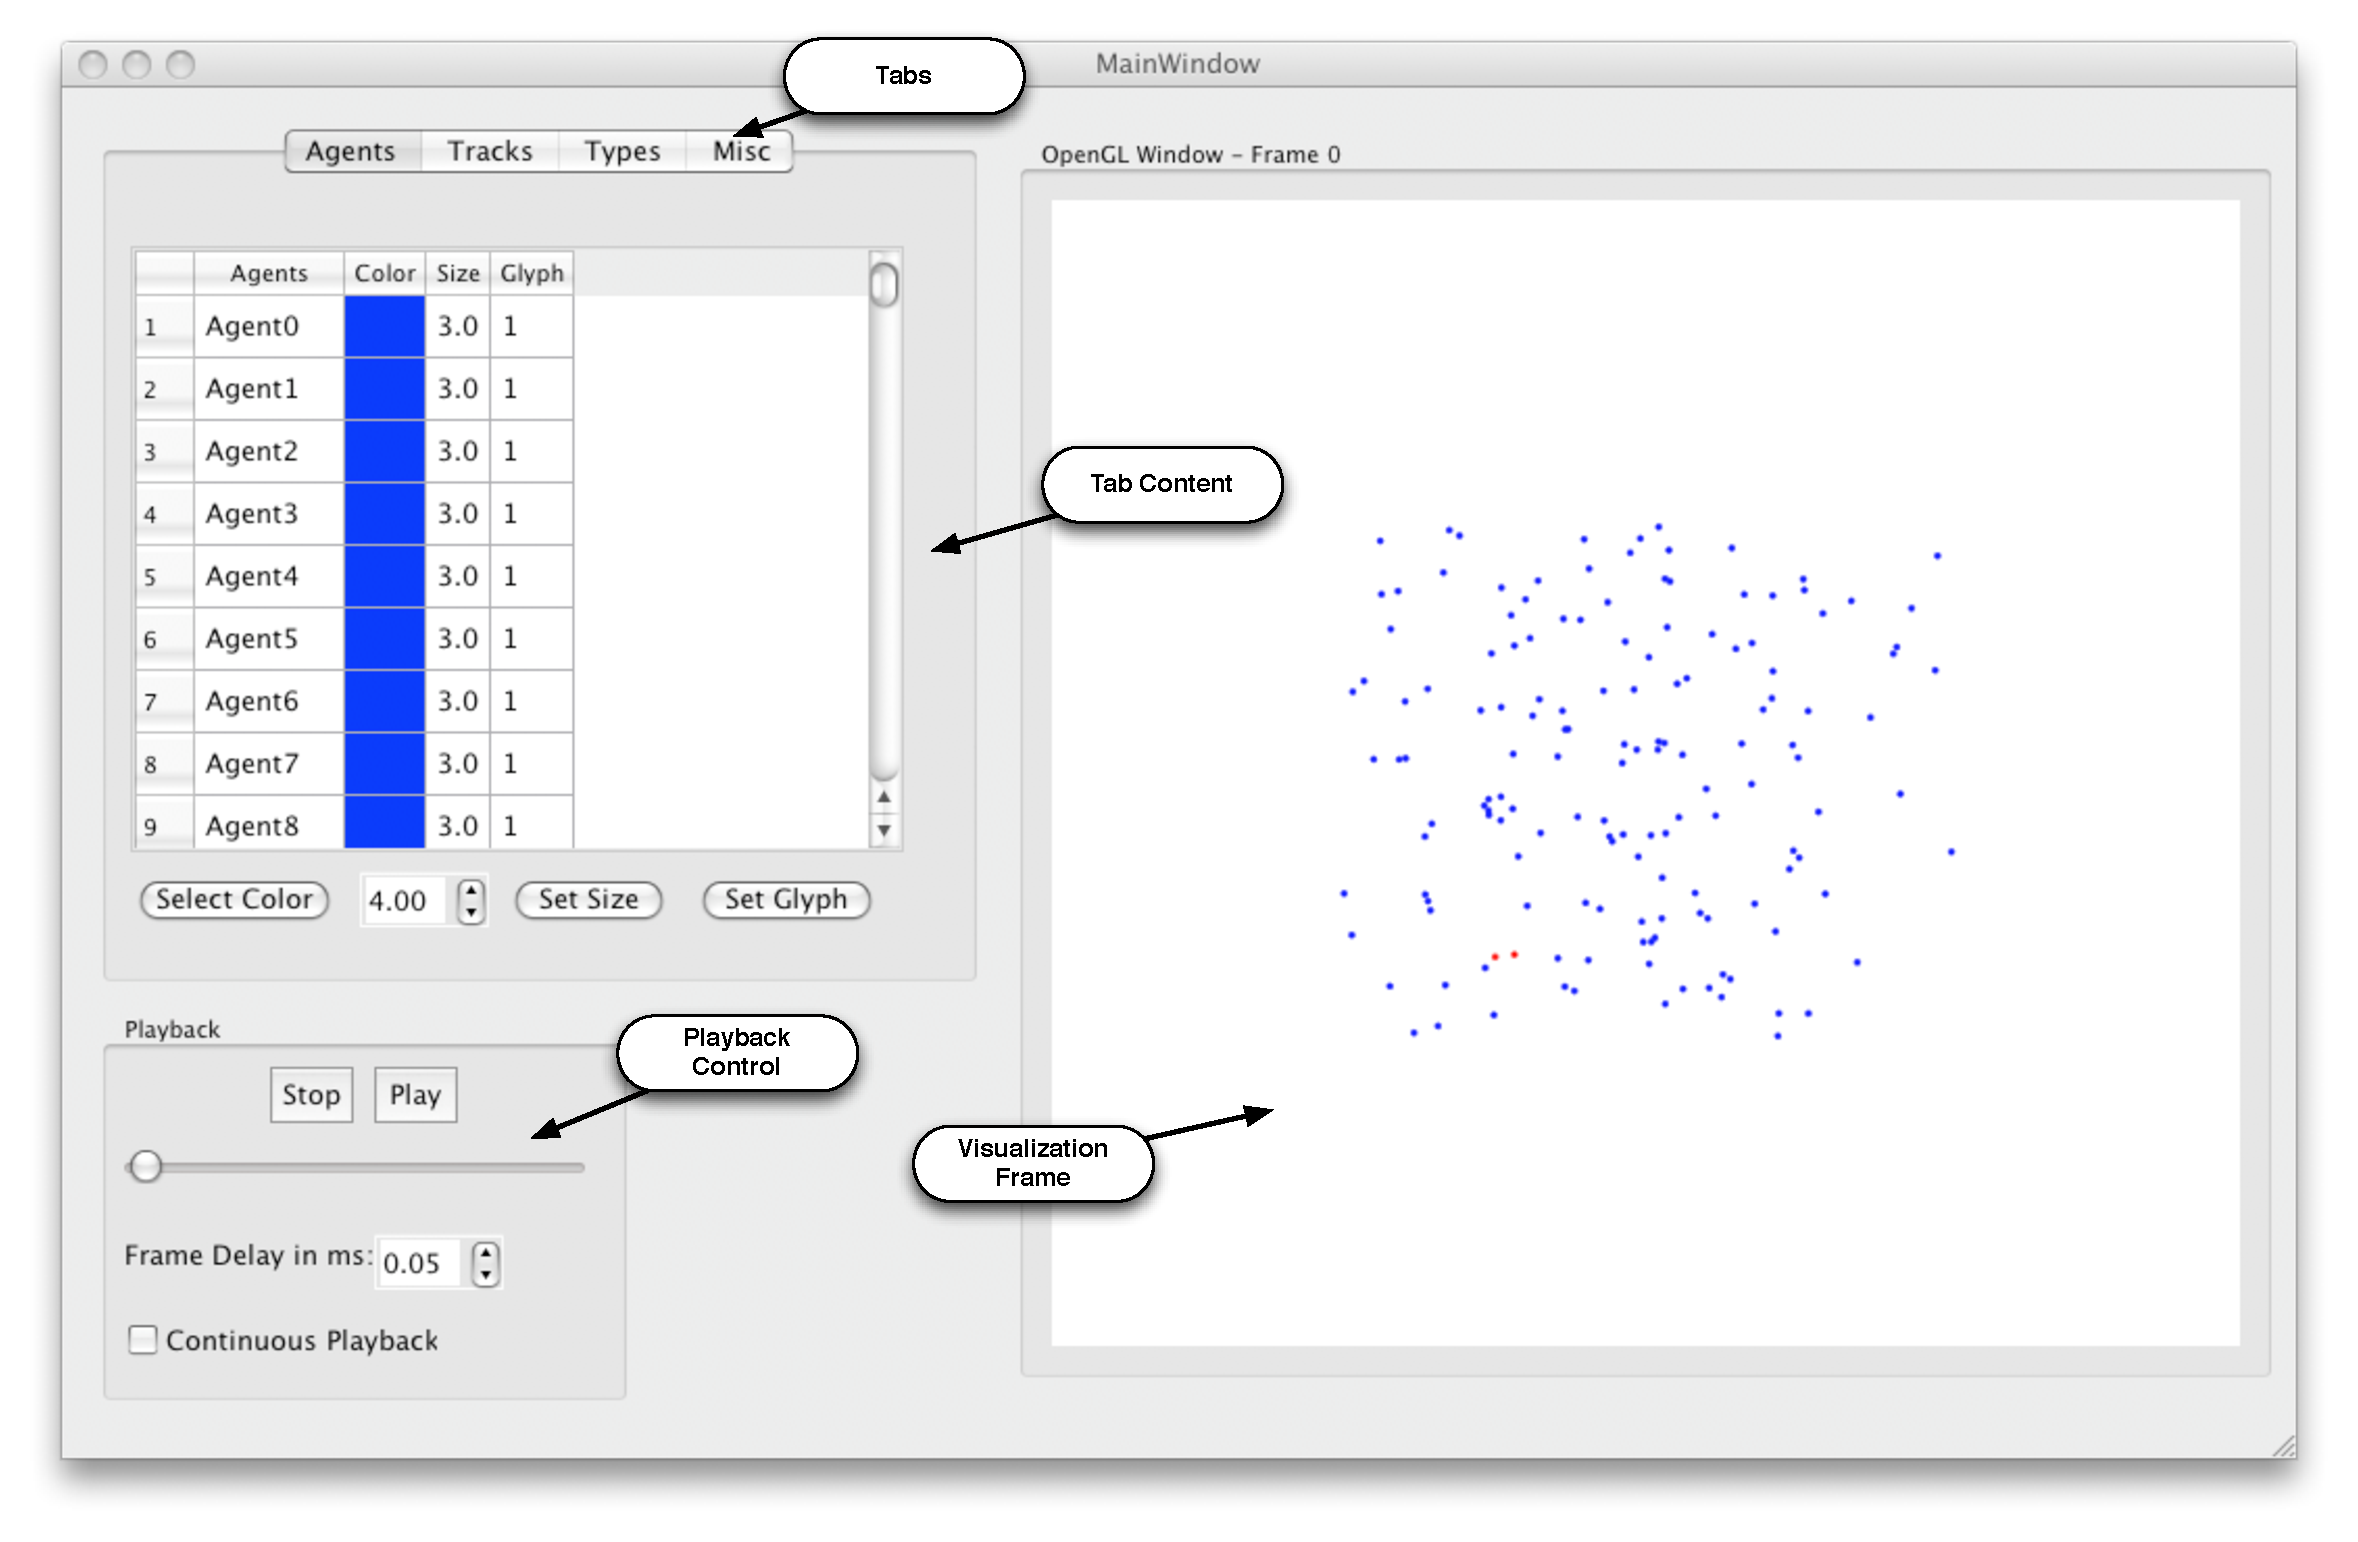
\includegraphics[scale=.45]{images/swarmvis-annotated.pdf}
\caption{The SwarmVis graphical user interface. 
The interface is split between the user controls (left) and the visualization (right). There are tabs at the top left that give
options for different visualizations in the tab content frame. The playback frame in the bottom left works similar to a
standard media player. The visualization frame shows the swarm with all selected visualizations applied to it. In this
screenshot, the user has two agents colored red with all no other options enabled. A file menu (not shown) allows for loading swarm datasets.}
\label{AnnotatedWindow}
\end{figure*}

\section{Implementation}
SwarmVis is implemented in the C++ language and utilizes the Qt framework\cite{Qt:website}
to build the graphical user interface. The OpenGL library is used to render all visualizations. The choice of software libraries facilitates cross-platform utilization of the toolkit.
The user interface is divided into a settings/options frame and visualization frame (see Figure \ref{AnnotatedWindow}).
The settings/options frame (left) contains the majority of the user interface, whereas the visualizations frame (right) contains  the graphical display.
The visualization frame can be rotated and zoomed by dragging and scrolling a mouse, respectively.
In general, we kept the interface as simple and straightforward as possible.
A more detailed description of the user interface is given in Figure \ref{AnnotatedWindow}.
Changes made to the visualization through the interface are applied to any visualization in real-time.
Lists and parameters are populated when a data set is loaded (more information about data sets is available in the appendix).

Still images can be created by SwarmVis by dumping the graphic currently shown in the visualization frame.
Also, videos can be made by having SwarmVis automatically dump every frame in the course of an animation as an image.
These images can then be compiled into a video by a third-party program that is used to make stop-motion or time-lapse
videos.\footnote{Boid flock and tetrahedron-forming swarm videos made by SwarmVis:\\
 http://maple.cs.umbc.edu/~don/projects/SAF/videos/\#tetra}

In the remainder of this section, we list the available visualizations in SwarmVis, what they convey, how they are implemented,
how they can be enabled, and how they can be modified.


\subsection{Visualizations}\label{visualizations}


\begin{figure}
\centering
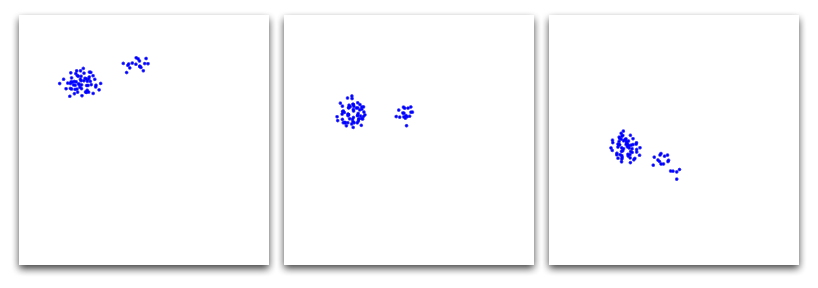
\includegraphics[scale=.282]{images/animation.png}
\caption{
Three captured frames from a swarm animation of three-dimensional flocking boids\cite{reynolds1987}.
When viewed in quick succession as frames in a video, the user
is able to detect the flocks' motion and structural changes.}
\label{Animation}
\end{figure}

\subsubsection{Animation}

The playback control (as seen in  seen in Figure \ref{AnnotatedWindow})
gives the user the ability to specify what time step is being shown in visualization frame.
The inspiration for this control is a standard media player such as QuickTime Player or Windows MediaPlayer.
The control provides the ability the ability to stop,
play and manually move through frames (with the slider).
In addition, the user can specify how fast the animation is created by adjusting the amount of delay between
frames (``frame delay" box).

Viewing a swarm over several time steps conveys a great deal of information. It conveys direction,
velocity and structure by displaying how the swarm changes from time step to time step.
SwarmVis manages to make these animations incredibly smooth on a modern
computer,\footnote{2.2 GHz MacBook Pro running Mac OS X 10.5} even with a fast frame rate and hundreds of agents.
An example of this is shown in Figure \ref{Animation}, in which a swarm is shown to be
generally moving south with its sub-swarms beginning to merge.
All of the SwarmVis visualizations  that can be applied to the swarm (color, size, trails, tracks) can be seen in fluid animation.








\begin{figure}
\centering
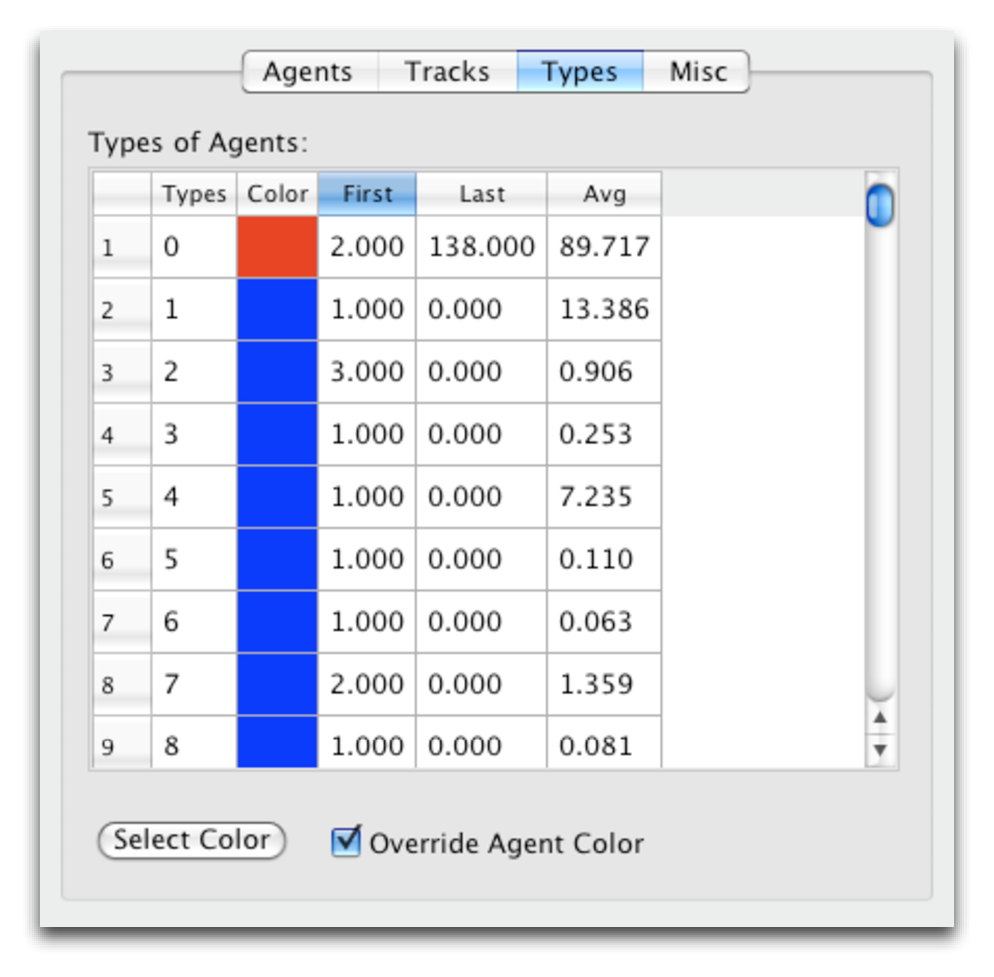
\includegraphics[scale=.5]{images/typestab.pdf}
\caption{
The Types tab shows the user which different subgroups exist in the swarm and allows the user to assign a specific
color to that group. Supplemental information helps the user
select the groups he wants: First (number of agents in that group in the first frame),
Last (number of agents in that group in the last frame), and Avg (average number of agents in that group during
the entire animation).}
\label{TypesTab}
\end{figure}

\begin{figure}
\centering
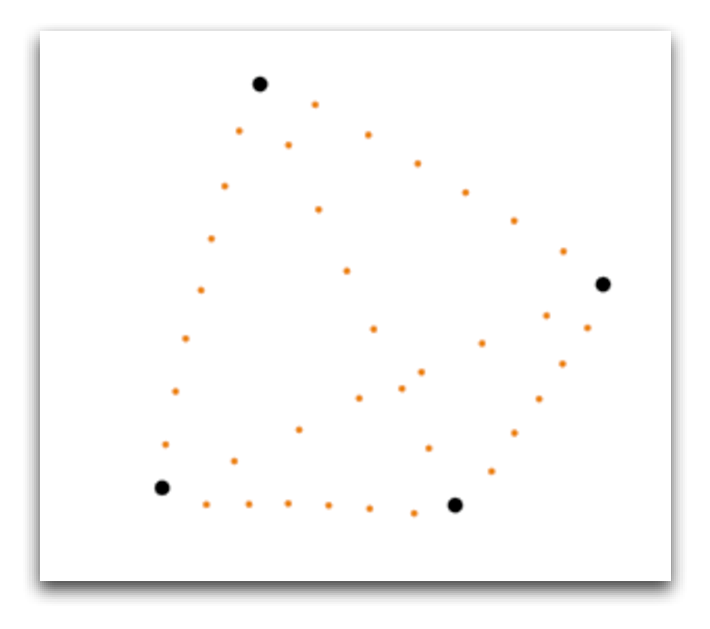
\includegraphics[scale=.4]{images/sizeandcolor.pdf}
\caption{
A captured frame from a swarm of tetrahedra-forming boids.
The corner agents have been given a larger size and a darker color than the edge agents.}
\label{SizeAndColor}
\end{figure}


\begin{figure}
\centering
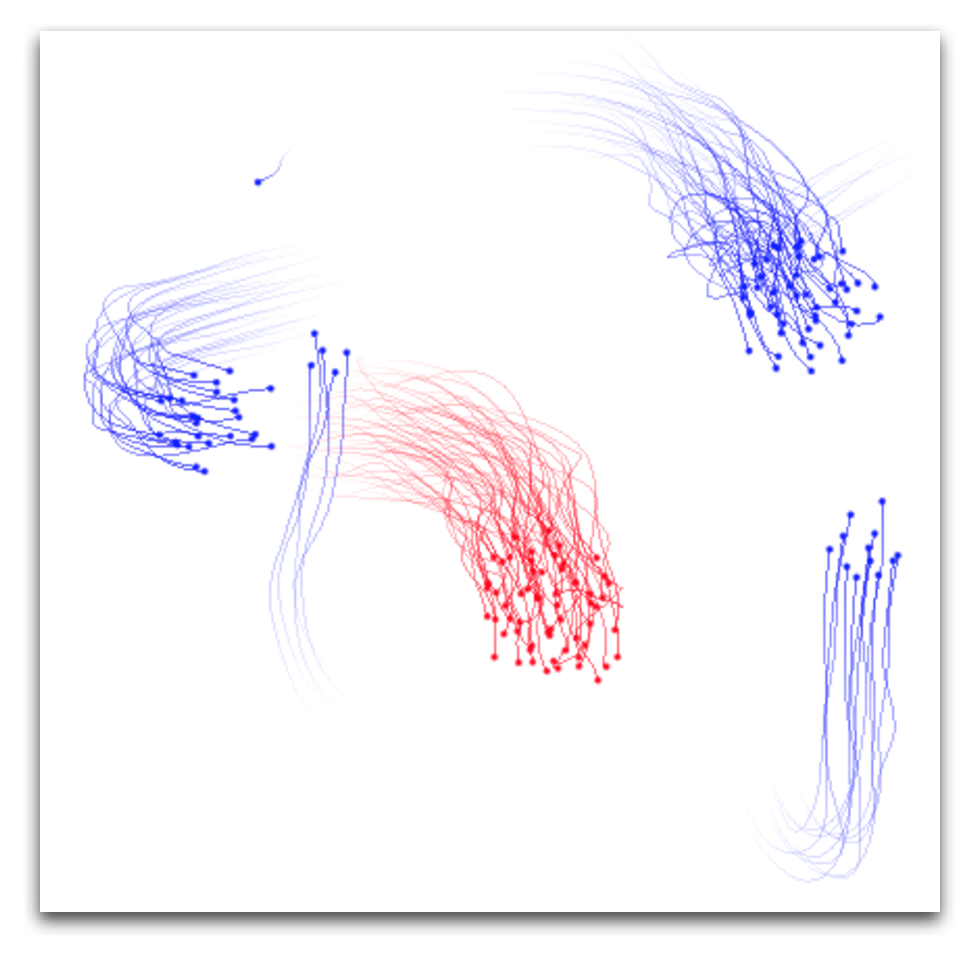
\includegraphics[scale=.45]{images/flockcolor.pdf}
\caption{
A captured frame from the three-dimensional flocking swarm shown in Figure \ref{Animation}.
The trails in this image are of length 35 time steps and agents of a particular group are colored red.}
\label{FlockColor}
\end{figure}


\subsubsection{Color and Size}

An important feature of SwarmVis is the ability to track individual agents.
This can be done by selecting any number of agents of interest in the list of agents
(seen in the content frame of Figure \ref{AnnotatedWindow})
and changing their color or size with the button controls.
For example, in Figure \ref{SizeAndColor}, the some agents have been made bigger to emphasize their importance.

In addition, users can change the color of all agents that are members of a specific group in the \textit{Types} tab, as seen
in Figure \ref{TypesTab}.
This feature can be used in conjunction with size changing to emphasize particular agents.
For example, in the swarm shown in
Figure \ref{SizeAndColor}, we color the corners \textit{black} and the edges \textit{orange}. Another
example is shown in Figure \ref{FlockColor}, in which the largest flock of agents is colored \textit{red}. The remaining agents are colored in \textit{blue} (default color).
Changing the color of the largest flock in the flocking domain is
particularly useful because it shows when two groups merge by changing the agents' colors
as they collide.
Also, this feature is great for creating figures for swarm research articles because
by changing the color and size, the author can refer to specific agents as ``the bigger agents"
in the text instead of having to manually add labels to the images.





\begin{figure}
\centering
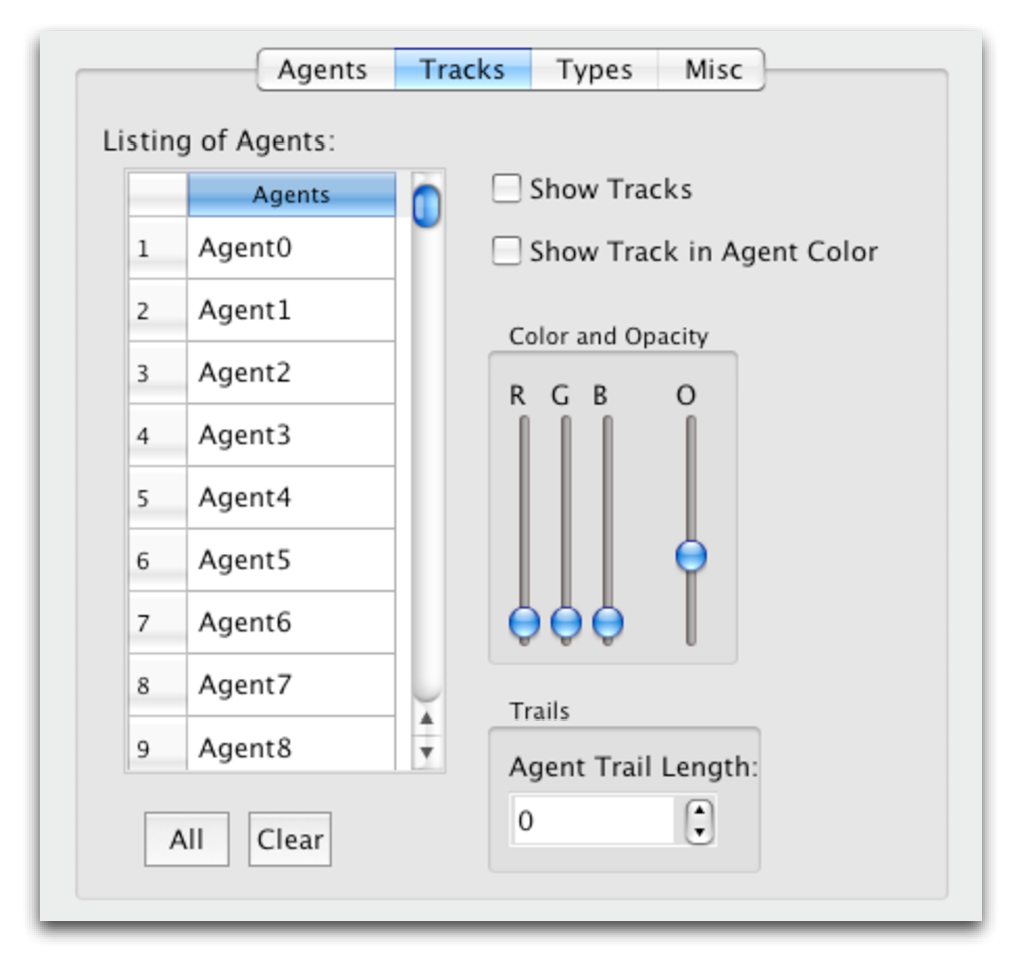
\includegraphics[scale=.5]{images/trackstab.pdf}
\caption{
The \textit{Tracks} tab allows users to add tracks and trails to agents. The length of the trails can be adjusted 
with the ``Agent Trail Length" box. }
\label{TracksTab}
\end{figure}

\begin{figure}
\centering
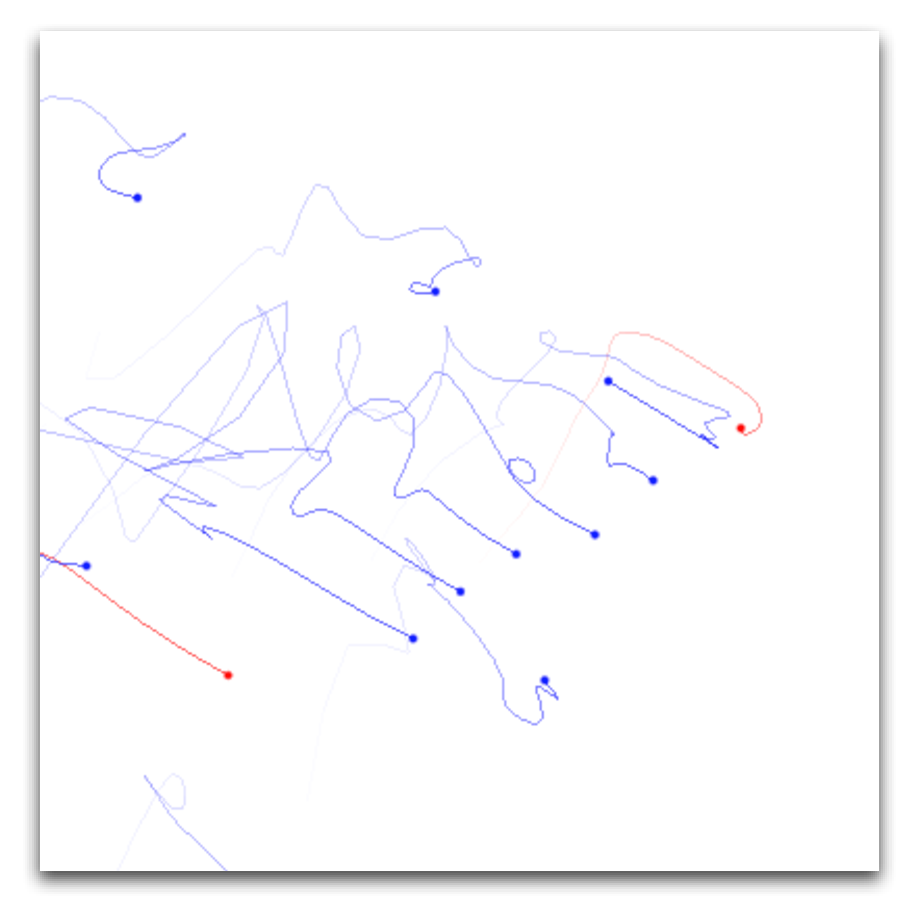
\includegraphics[scale=.5]{images/closeuptrails.pdf}
\caption{
A captured frame from a swarm of tetrahedra-forming boids shown in Figure \ref{SizeAndColor}.
Close up views of the swarm can convey much information about how agents interact with one another.
In this frame, we see how the right-most red corner agent swapped places with the rightmost edge agent.
Then, edge agents fill in the gap by moving to the right. The different times in which each adjustment happened
is shown by how long ago a pattern happened in the trail.}
\label{CloseTrails}
\end{figure}

\subsubsection{Trails}

Trails are one of the most important features in SwarmVis because they convey motion, previous positions, direction,
and change in structure. This fact applies equally to still images and videos. Trails are lines that hang behind agents, tracing
their previous positions. 
The trails are created by connecting previous positions of the agents with
successive lines that are more opaque near the head of the agent and less so further back in time.
The length of trails can be adjusted by modifying the number in the ``Agent Trail Length" text box, shown in
Figure \ref{TracksTab}.

Trails can be used to view swarm behavior at an abstract level, such as tracking the motion of several boid
flocks at once, as seen in Figure \ref{FlockColor}.
One of the most powerful abilities of trails is to convey low-level behavioral information in swarms. For example,
in Figure \ref{CloseTrails}, we can see that the right-most corner agent (colored red) swapped position with the right-most
edge agent (colored blue). Then, all the agents in that edge shifted down to accommodate.
The time delay in behavior is shown by the ``notch" in the path happening further back in time for the left agents, and more recently for the right agents.
This visualization feature makes qualitative analysis of agent behavior possible - both at a low interaction level
and a high emergent level.







\begin{figure}
\centering
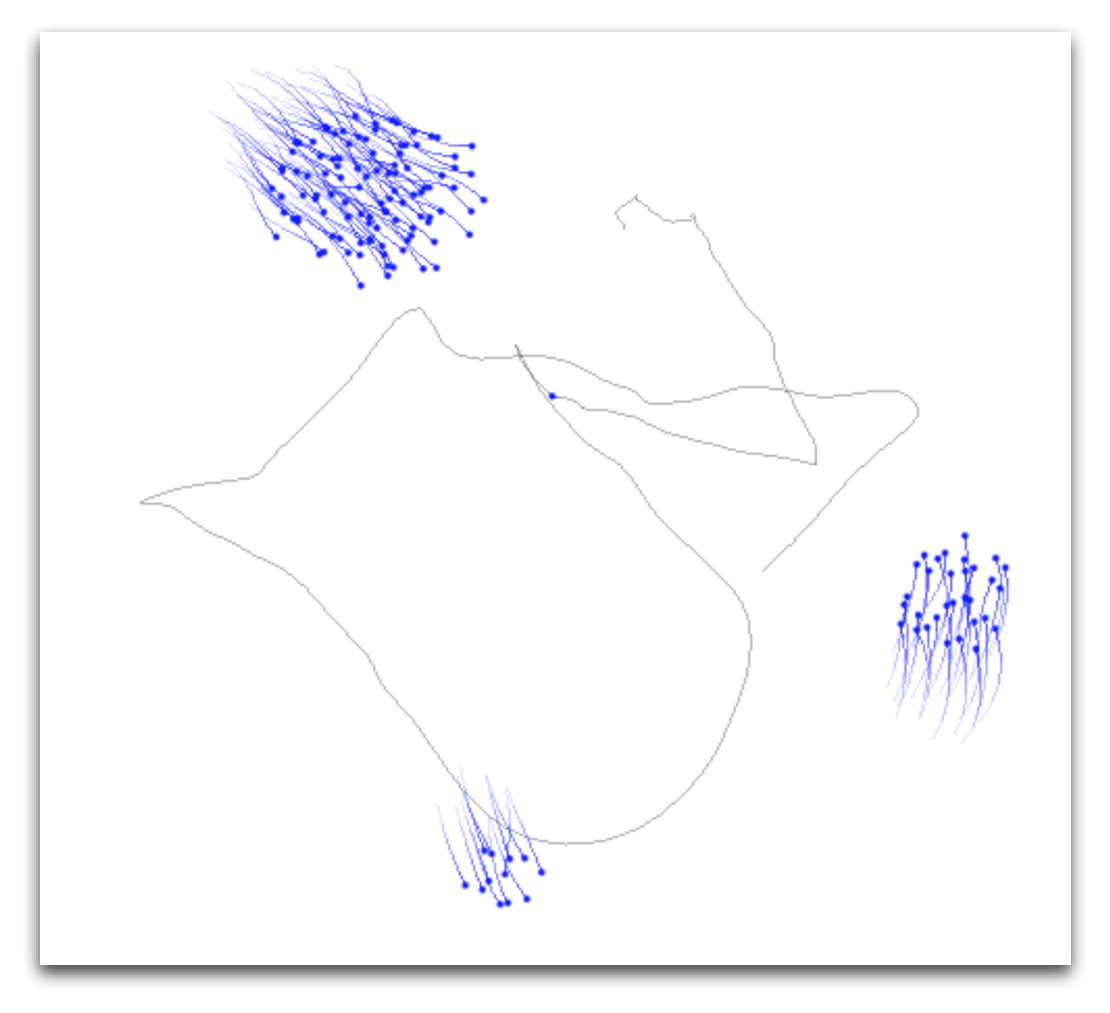
\includegraphics[scale=.4]{images/track.pdf}
\caption{
A captured frame from the three-dimensional flocking swarm shown in Figure \ref{Animation}.
The lonely agent (marked by being larger and darker) in the middle follows this path over its lifetime.
The path is colored based on velocity, showing that it moved rather slowly while being solitary (blue portion).
The agent then sped up after being picked up by a flock (red portion). This event is inferred by the ``notch,"
as well as the change in color between the blue path and the red path.
The structure of the line in three-dimensional space is more apparent when a user interactively rotates the visualization frame.}
\label{Track}
\end{figure}


\subsubsection{Tracks}

The tracks feature is very similar to the trails feature. Unlike trails, tracks show the position of an agent over the entire
lifetime of the system. At any given frame, the agent can be found at its respective position on the track.
For example, a track of a single agent is shown in Figure \ref{Track}.
Several agents can be selected at once in the list of agents in the \textit{Tracks} tab (Figure \ref{TracksTab}) to
have all their trails shown at once.
When tracks are used in conjunction with trails, the trails are overlaid on top of the tracks so that
both trail and track information is conveyed.





\begin{figure}
\centering
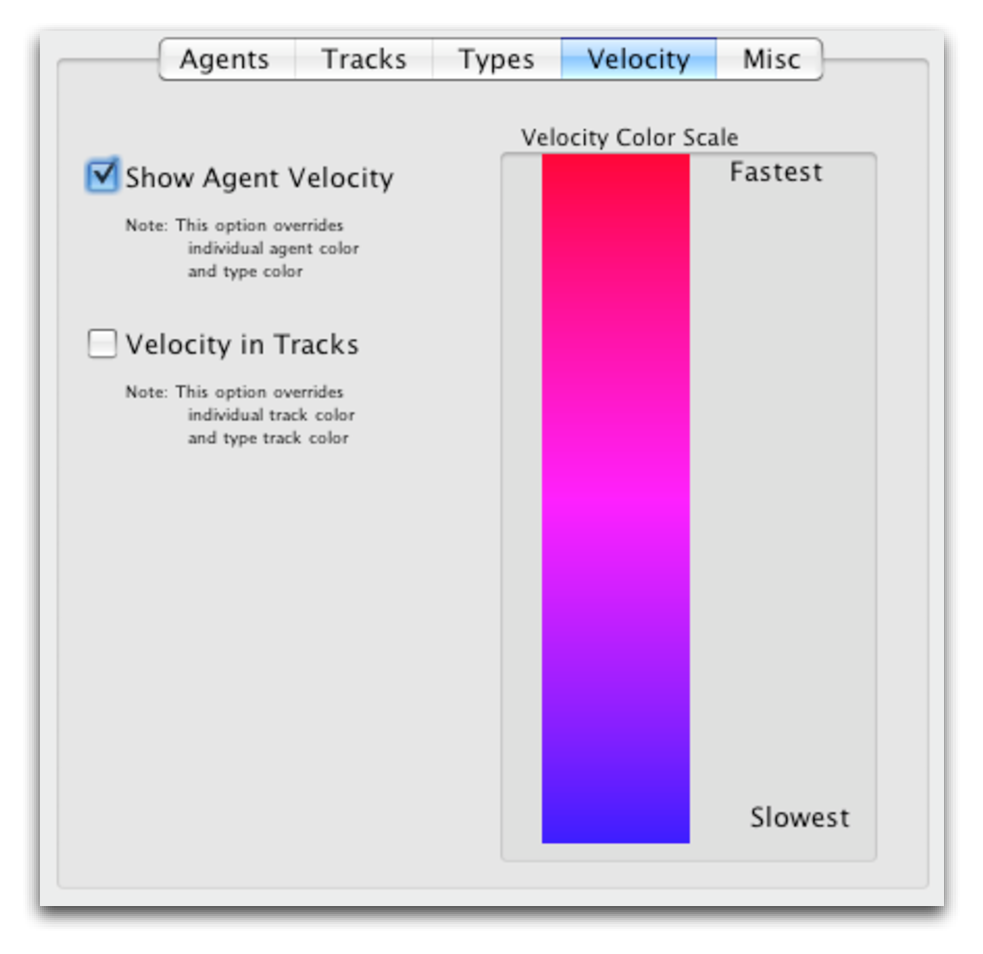
\includegraphics[scale=.5]{images/velocitytab.pdf}
\caption{
The velocity tab allows users to map agents' velocities to a color, shown in the gradient on the right. The ``Show Agent Velocity"
option will color the agent and its entire trail (if enabled) more red if the agent is moving relatively fast, or more blue if the agent
is moving relatively slow (seen in the right image of Figure \ref{Velocity}).
The ``Velocity in Tracks" option makes it so the agent tracks are colored according to speed at that time step (seen in the left
image of Figure \ref{Velocity}).}
\label{VelocityTab}
\end{figure}

\begin{figure*}
\centering
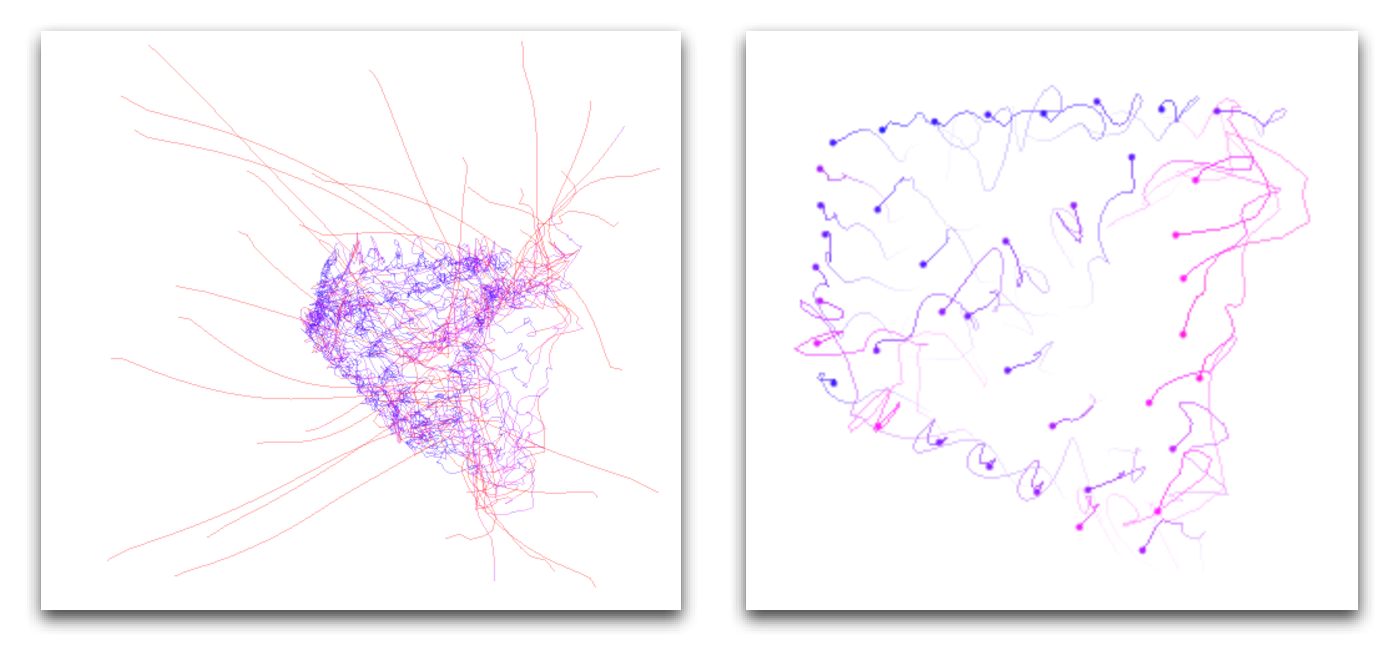
\includegraphics[scale=.666667]{images/velocity.pdf}
\caption{
A captured frame from a swarm of tetrahedra-forming boids shown in Figure \ref{SizeAndColor}.
On the left, all agent tracks are displayed, showing that agents move faster (the color red) at the beginning.
Once the agents organize into the tetrahedron they slow down (the color blue).
On the right, the trails and the agents themselves are colored according to their instantaneous velocity.
From this captured frame, it is obvious that the right edge is experiencing movement while the rest of the
shape is calm. }
\label{Velocity}
\end{figure*}

\subsubsection{Velocity Color}

The velocity feature is useful for displaying the instantaneous or historical velocity of agents.
This visualization can be applied in two different ways: (1) color the agent and its trail the agent's current instantaneous
velocity and/or (2) color the agent tracks based on the velocity at each time step on the track.
SwarmVis uses the distance travelled in one time step to determine the velocity of an agent and then calculates the 
desired color from a color gradient.
The default color gradient is determined by making pure red the greatest velocity seen in the data set and making pure blue
a velocity of zero (as seen in Figure \ref{VelocityTab}).

By coloring agents based on instantaneous velocity, while viewing the swarm as an animation,
change in velocity is conveyed by change in color.
In addition, important information can be gleaned by viewing still images of agents colored by velocity:
Agents that are moving faster are colored differently than agents that are moving slower.
An example of this is shown in Figure \ref{Velocity} (right).
We decided that coloring the entire trail the instantaneous velocity (opposed to its default color)
makes the color more obvious.
There is no actual information contained in the trail's color, as it is the same color as the agent.

Coloring tracks based on the velocity is a powerful feature that displays how an agents' or an entire swarm's
velocity changes over the course of the system.
Every line segment in the track is colored based on the velocity of the agent on that line segment.
A single agent's track is pictured in Figure \ref{Track}, in which we see how the velocity of this particular agent changes
over the course of its lifetime.
In contrast, in Figure \ref{Velocity} (left), every agent has its track shown.
From this image, we can determine that the movement is very fast and chaotic in the initial phases but then calms to a slower
speed, once the agents have organized into the shape.

\section{Results: Analysis of the Tetrahedron-Forming Swarm}

Throughout the course of this document, we have discussed the motivation behind the visualizations in SwarmVis by
displaying images from two data sets: a boid flock and a tetrahedron-forming swarm.
In this section, we provide a cohesive and comprehensive walkthrough of how a user would
analyze the tetrahedron-forming swarm.

\subsection{Background}

The shape is formed by agents adhering to the following procedure.
First, four corners are selected by the swarm via a simple election algorithm.
Then, the agents persistently execute the following rules:
\begin{itemize}
	\item If a corner, be attracted slightly to the three other corners.
	\item If not a corner, be attracted to the two closest corners with great, but equal, strength.
	That is, the output force vector of this rule is the sum of two vectors with some constant magnitude.
	Note that when an agent is on the line formed by its two closest corners, the forces cancel each other out.
	\item Move away from any agents that get too close.
\end{itemize}

The end result of these rules are somewhat obvious: the agents self-organize into a tetrahedron.
However, many of the fine-grained details of the agent behavior is not clear.
For example, some questions one may want to ask about this system are: 
\begin{itemize}
\item Will the shape formed be equilateral?
\item How stable is the shape once it is formed? Does it reach an equilibrium and stop moving? If not, what is changing?
\item How do agents react to movement in the tetrahedron?
\item How fast do agents create a shape that appears to be a tetrahedron?
\item Are there any interesting ``emergent strategies" that this swarm uses to create the shape?
\end{itemize}
These questions and  more are not easily answerable by studying the rules or the raw position data.
The purpose of SwarmVis is to provide users the power to answer these questions,
as well as identify emergent behaviors not previously expected to exist in some systems.

The particular tetrahedron-forming swarm data set we will be analyzing in this section has forty agents
and is comprised of 333 individual frames of agent coordinates.

\subsection{SwarmVis Analysis}
SwarmVis has several tools available to analyze swarms and create informative visualizations.
To demonstrate the results of our work, we provide examples of how the tetrahedron-forming swarm can be analyzed.
The three general approaches discussed in this section are only a starting point in studying this domain.
Due to the nature of these complex systems, there is always something interesting waiting to be found.
SwarmVis enables the user to discover these points of interest, which otherwise would be undiscoverable.


\begin{figure}
\centering
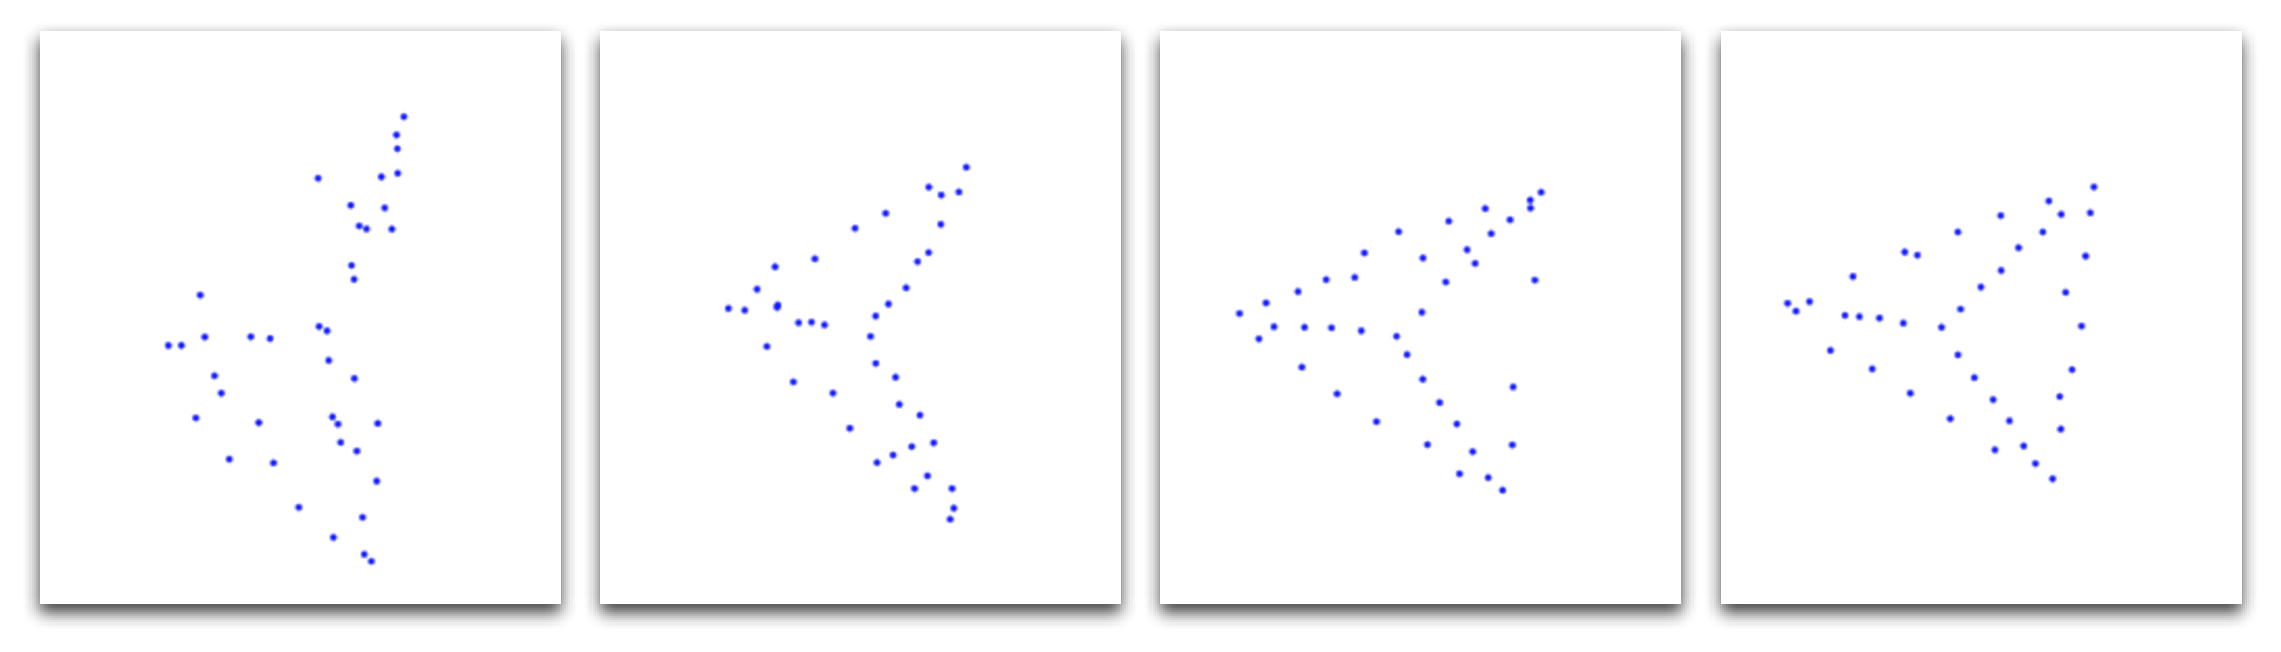
\includegraphics[scale=.21]{images/tetraclosing.pdf}
\caption{
The tetrahedron-forming swarm uses an emergent strategy to form its last (sixth) edge.
The swarm initially form two triangles with a shared edge (total of five edges), then
close in on itself to form the last edge. This is easily seen by watching the swarm in animation.}
\label{TetraClosing}
\end{figure}

\subsubsection{Animation}
Several interesting observations can be made by viewing the swarm with an animated series of plotted points.
From an animation of the tetrahedron-forming swarm,
we immediately determine that the swarm starts out spread thin with no organization.
Then, agents move towards the center and follow an emergent strategy (i.e., not explicitly part of the agent rules)
to form the sixth edge of the tetrahedra: form two triangles with a shared edge (five edges) then loose two corners
in on themselves, forming the sixth edge. Agents executing this strategy are shown in Figure \ref{TetraClosing}.
After this, we can see the swarm moving towards the center of the screen in a stable manner.
Then, all of a sudden, agents start bouncing back and forth from edge to edge, not permitting the tetrahedron to
reach an equilibrium.
Other than these obvious facts, not much more information can easily be inferred by watching this simple animation.

Our first step in making more useful visualizations is to color the corners differently than the rest of the agents so that
they are easier to track. We see in the Types tab (Figure \ref{TypesTab}) that there are two groups, labeled
``corner" and ``edge" (agents are explicitly labeled in the data set).
Although the labels are intuitive, we can also infer that the second group in the list
contains the corner agents because it has an average of 3.988 member agents over the lifespan of the swarm.
Since a tetrahedron has four corners, it is safe to assume that this group contains the corners we wish to color.
This feature is important in this domain because the corner agents follow different
rules than the edge agents.
Therefore, segregating them will make it easier to understand how the swarm functions.
At this point of the walkthrough, our visualization shows a tetrahedra similar to that in Figure \ref{SizeAndColor}.

The best way to share animations is to create a video with SwarmVis.
Videos would be appropriate for sharing information conveyed by an animation online or in presentations.

\begin{figure}
\centering
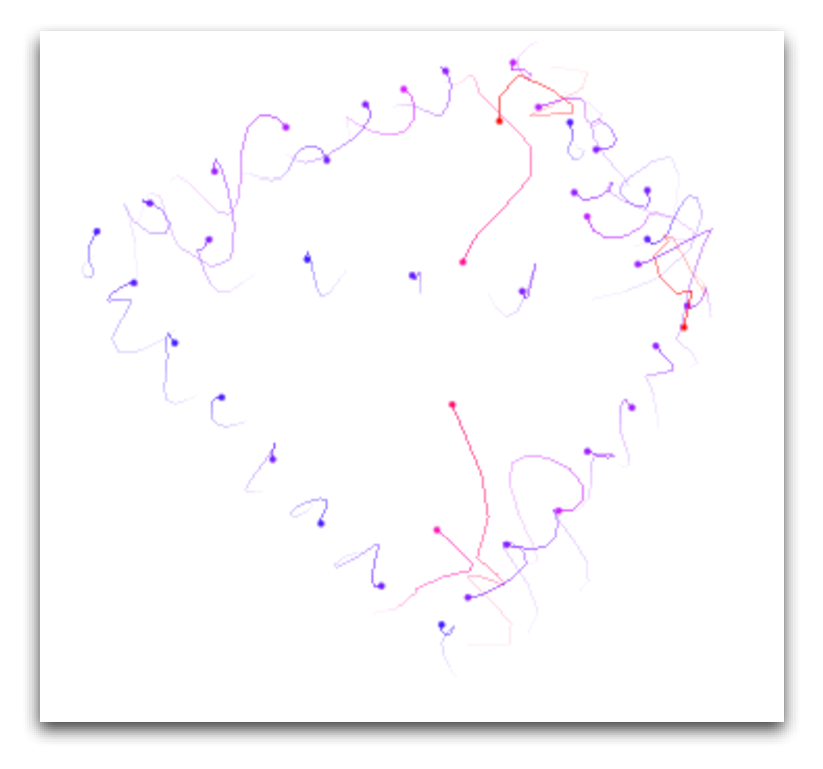
\includegraphics[scale=.55]{images/tetrastrategy.pdf}
\caption{
The tetrahedron-forming swarm creating its sixth edge with velocity-colored trails enabled.
}
\label{TetraStrategy}
\end{figure}

\subsubsection{Trails}
Previously, in Figures \ref{CloseTrails} and \ref{Velocity}, we described how trails can convey important information.
We now add another example of how powerful of a tool agent trails are in creating compelling still images.
Velocity-colored trails can be used to explore how the tetrahedra-forming swarm is completing the sixth edge of the shape.
The trails show where the agents are coming from and where they are going.
Also, with velocity coloring we can easily see which agents are shifting significantly.
By zooming in close to the sixth edge as it closes and taking a still image at the appropriate time (which we found
with moving our slider slowly), we receive the image shown in Figure \ref{TetraStrategy}.
From this image, we can tell that the edge agents closest to the corners are the ones that form the new edge.
These agents move very quickly, as seen by their red coloration.
Meanwhile, agents from the edges these quick agents are coming from shift to fill in the gap.
These agents are colored purple due to their relatively slower movement.
At this point, we feel we have a detailed understanding of how the last edge is formed through this emergent strategy.
Without trails, this phenomena could not have been demonstrated in a single image (e.g., see Figure \ref{TetraClosing}).



\begin{figure}
\centering
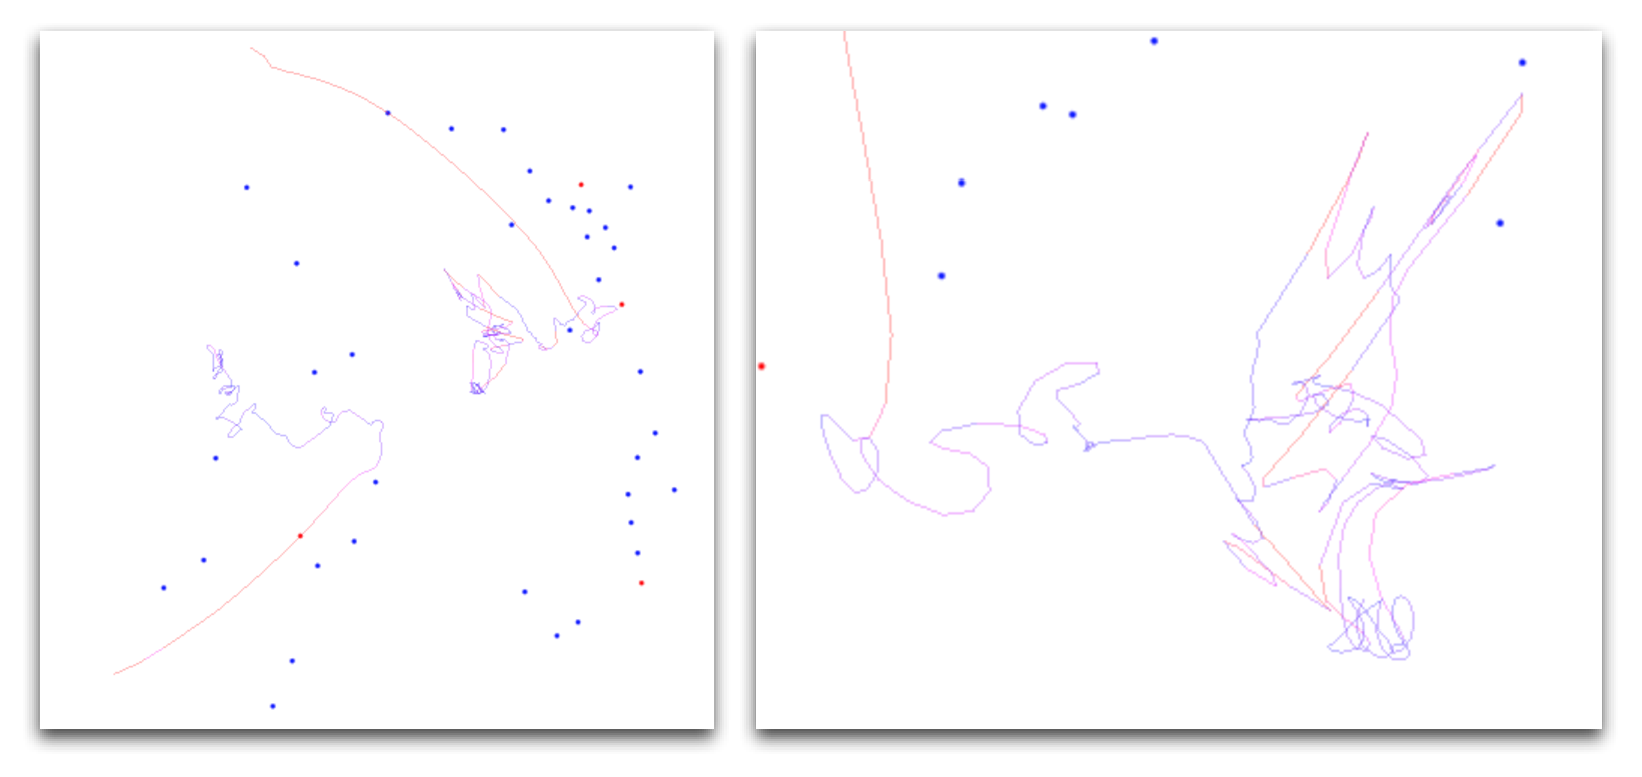
\includegraphics[scale=.3]{images/cornervsedge.pdf}
\caption{
(Left) A comparison of a corner's track and an edge agent's track.
The two can be contrasted by analyzing the color and structure of the tracks.
The corner agent gets into position and remains relatively calm for the remainder of the time.
(Right) Meanwhile, the edge agent goes through several high-speed moments and never reaches a steady state.
}
\label{CornerAndEdge}
\end{figure}

\subsubsection{Tracks}
Previously, in Figure \ref{Velocity}, we showed that velocity colored tracks can be used to get a high-level view of the swarm behavior.
Colored tracks can also be used to infer information about an individual agents' behavior.
To do this, we cycle through several agents listed in the Tracks tab.
Very quickly, we realize that there is a significant difference between the behavior of a corner agent and an edge agent.
A comparison of the two types of agents is given in Figure \ref{CornerAndEdge}.
From the image showed in this figure, we see that the life of an edge agent is far more chaotic than that of a corner agent.
The corner agent barely changes position after reaching its desired location,
while the edge agents movements are both highly variable in terms of position and velocity.
In some situations, selecting agents that end up neighbors can convey information about how they affect one another.







\section{Future Work}
We have demonstrated that SwarmVis is a powerful and dynamic tool.
It is a complete application that has accomplished all the goals that we set out to achieve. 
However, there are a few user interface changes that would make usability better.
Also, we would like SwarmVis to visualize the instantaneous velocity and the depth of
agents since this information is not explicitly present in the
graphical display. These future improvements are discussed in this section.

In the future, we would like to make it easier to select agents and determine which agents are which in the graphical display.
To facilitate this, we hope to be able to show text labels that are adjacent to the agent in the visualization window.
These labels can show the name of the agent in the agent list.
Also, the ability to click agents in the visualization window will allow for greater interactivity and easier modification of agent-level colors and effects.

Currently, each visualization effect is controlled by a separate procedure.
Therefore, separate agent lists are kept in the Agents tab, the Tracks tab and the Types tab.
To make changes to an effect requires using that effect's tab and any changes made (e.g., color) are not reflected in the other lists.
Having an interactive global agent list that displays all necessary information will enable users to modify
the colors and effects on groups of agents more effectively. 

We also plan on adding the feature to change the representation of the agent itself to better display direction. Currently, direction is
inferred by the user by viewing the agents' trail, which may not be effective in every situation.
If agents were represented as three-dimensional arrowheads or perhaps other glyphs,
still images would convey very clearly the direction the agent is going on.

To further enhance the information conveyed in still images, we plan on determining a sufficient way to display depth.
We are not sure what the best technique for this would be, and no previous work to our knowledge has specifically dealt with this problem.

Finally, we plan on making SwarmVis extendable through a plug-in type framework. Any new visualization effects that are added
to SwarmVis must be hard coded into the source. This is not intuitive for a user that does not have knowledge of the source code
who wishes to add his own visualization to SwarmVis. Plug-ins could be simple programs that take the agent data as input and return
what the plug-in would like to have drawn on the screen. For example, the agent trails effect could be implemented as a plug-in, such
that it returns a list of lines to be drawn. A plug-in user interface will have to be implemented that allows users to manage plugins,
as well as use them. There should be some way for the plug-ins to interface with the global agent list to add informations to columns
and access information.


\bibliographystyle{IEEE}
\bibliography{cmsc636-swarmvis}

%\vspace{500pt}

\pagebreak

\appendix[User Guide]

\subsection{Compiling and Running}
SwarmVis was created to run on Unix-like systems, such as Mac OS X and GNU/Linux.
The following programs are required to compile SwarmVis:
\begin{itemize}
\item Qt 4.2
\item gcc/g++ 4.2.2
\item make
\end{itemize}
Note that some libraries from Qt4.2 may be needed to run SwarmVis in binary form.
We have tested SwarmVis on Mac OSX 10.5 and openSUSE Linux 11.

Run \texttt{qmake}, then run \texttt{make}, both in the root directory, to compile SwarmVis.
A binary will be created in the \texttt{bin/} directory. Execute this binary to run SwarmVis.

\subsection{Data File Format}
SwarmVis requires a specific file format for data sets that are to be loaded. The agents' position data is segmented into
separate files that each represent a single time step. These files are space-delimited data, with
each row representing an agent. For example, a swarm system with 100 agents depicted over 500 time steps
will have 500 files in a folder, each with 100 lines.

Each row entry in a file follows a format as well. The first two or three  columns (depending on dimensionality) are the
position data $(X, Y)$ or $(X, Y, Z)$, respectively. The last column is reserved for the group label, which may be used to pass
group membership data to SwarmVis.
For example, a well-formed line that conveys a three-dimensional
position with group information could be:
\begin{quote}
\texttt{10.15 5.24 84.85 CornerAgent}
\end{quote}
The listing of agents in each file should be stable. That is, the third line in one file and the third line in another file
should represent the same agent.

A plain-text information file containing important meta-data must accompany the frame files in the same directory.
The following variables must be defined (i.e., \texttt{VARNAME = VALUE}) in this file in order for the data to be loaded appropriately:
\begin{itemize}
\item \texttt{DIMENSIONS} (\texttt{2} or \texttt{3})
\item \texttt{AGENTS} (the number of agents)
\item \texttt{FRAMES} (the number frames/time steps)
\item \texttt{RANGEX} (the maximum X value)
\item \texttt{RANGEY} (the maximum Y value)
\item \texttt{RANGEZ} (the maximum Z value)
\item \texttt{AGENTTYPES} (\texttt{1} to track agent types, \texttt{0} if not)
\end{itemize}
At the bottom of this file, the keyword \texttt{FILES} must appear, followed by a list of frame files, in temporal order. The number
of files listed here must equal the number specified by the \texttt{FRAMES} variable. Also,
the number of lines in every file must match the number specified by the \texttt{AGENTS} variable. Below is a sample info file:
\begin{verbatim}
     DIMENSIONS = 3
     AGENTS = 150
     FRAMES = 446
     RANGEX = 600
     RANGEY = 600
     RANGEZ = 600
     AGENTTYPES = 1

     FILES
     frame000001.txt
     frame000002.txt
     ...
     frame000446.txt
\end{verbatim}

To load a data set in the SwarmVis application, navigate to ``Load Data" and select the info file.

\end{document}


